\chapter{Validaci�n y An�lisis de Resultados} %\index{Validaci�n}

A continuaci�n se muestran un conjunto de simulaciones realizadas en \textbf{Simulink} para analizar la efectividad de los diferentes esquemas de control definidos en la secci�n \ref{sec:Controlador-Capitulo-2} 

Las primeras tres simulaciones se realizan con el fin de comparar los diferentes controladores 

Las siguientes dos simulaciones tienen el fin de mostrar la efectividad del MCCE para reducir el consumo en los rodamientos radiales 


\subsection{Controlador retroalimentado vs Controlador integral} 

\begin{figure}[H]
\begin{center}
\centering
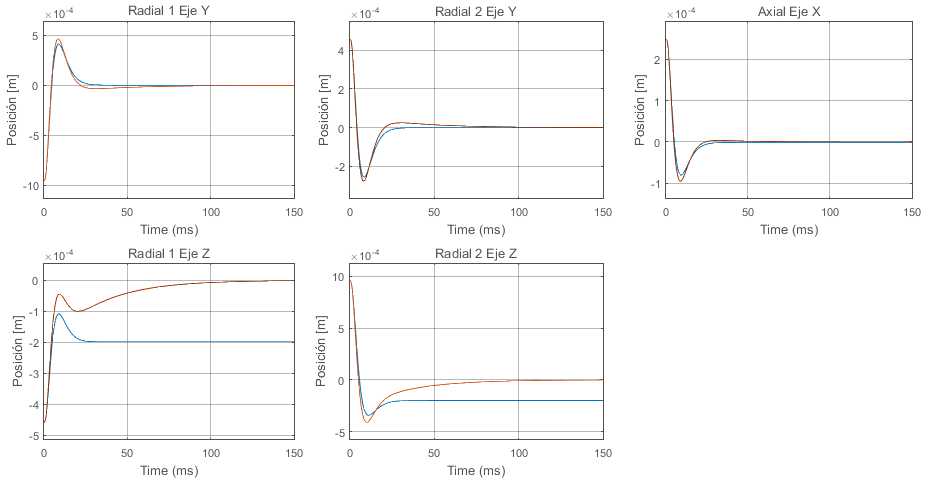
\includegraphics[width=\textwidth]{images/Capitulo_4_resultados_simulacion/simu_retroalimentado_vs_integral}
\caption{Controlador retroalimentado vs Controlador integral.}
\label{fig:Controlador_retroalimentado_vs_Controlador_integral}
\end{center}
\end{figure}

Se simulan dos controladores de tipo continuo 

[referencia controladores seccion 3.6]:  

\ref{fig:esquema-controlador-retroalimentado} y \ref{fig:esquema-controlador-integral}

ambos poseen un observador de estado en modo continuo 

la simulacion empieza con condiciones iniciales de ...

no hay carga ademas del peso del collar�n

como resultados el controlador retroalimentado nunca alcanza un error de estado estable igual a $0$ 

\subsection{Controlador continuo vs Controlador discreto} 

\begin{figure}[H]
\begin{center}
\centering
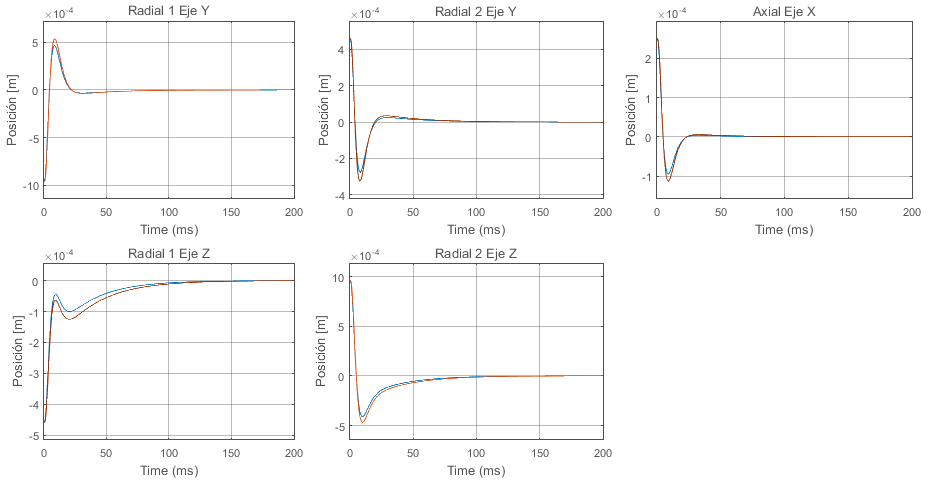
\includegraphics[width=\textwidth]{images/Capitulo_4_resultados_simulacion/simu_discreto_vs_continuo}
\caption{Controlador continuo vs Controlador discreto.}
\label{fig:Controlador_continuo_vs_Controlador_discreto}
\end{center}
\end{figure}

Se simulan dos controladores, uno de tipo integral continuo y otro de tipo integral discreto 

[referencia controladores seccion 3.6]:

\ref{fig:esquema-controlador-integral} y \ref{fig:esquema-controlador-discreto}

ambos poseen un observador de estado en modo continuo  y otro en discreto respectivamente

la simulacion empieza con condiciones iniciales de ...

no hay carga ademas del peso del collar�n

como resultados el controlador integral discreto emula bien al continuo

\subsection{Controlador linealizado en un punto vs calendarizado}

\begin{figure}[H]
\begin{center}
\centering
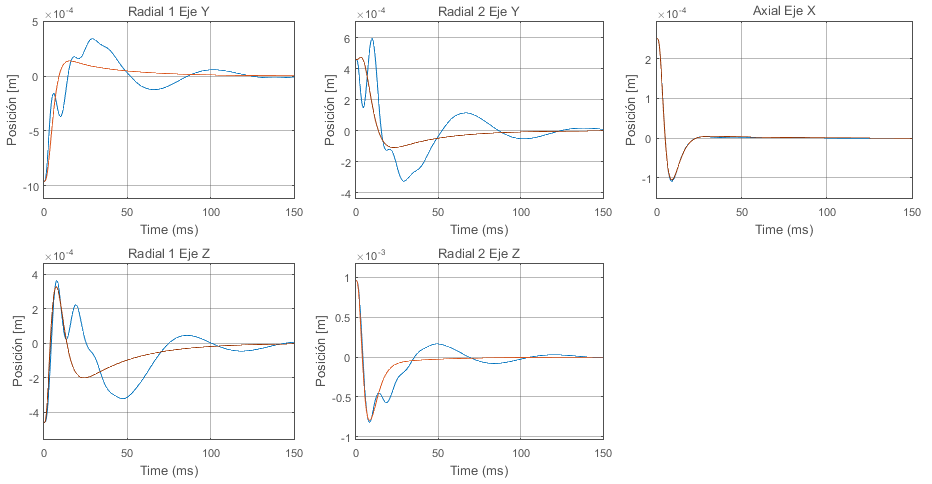
\includegraphics[width=\textwidth]{images/Capitulo_4_resultados_simulacion/normal_vs_calendarizado}
\caption{Controlador linealizado vs Controlador calendarizado.}
\label{fig:Controlador_linealizado_vs_Controlador_calendarizado}
\end{center}
\end{figure}

Se simulan dos controladores de tipo integral discreto linealizado en un punto y otro integral discreto calendarizado 

[referencia 3.6]:

\ref{fig:esquema-controlador-discreto} y \ref{fig:esquema-controlador-calendarizado}

ambos poseen un observador discreto y otro uno discreto calendarizado

la simulacion empieza con condiciones iniciales de ...

no hay carga ademas del peso del collar�n

cuando la velocidad angular del rotor es la misma que se us� durante el proceso de linealizacion ambos controladores operan de la misma manera 

cuando trabajan a velocidades angulares diferentes el controlador no calendarizado presenta problemas para estabilizar el rotor debido a los efectos de la precesi�n 

el control calendarizado no presenta problemas 

\subsection{Simulaci�n Accionamiento H�brido} 

\begin{figure}[H]
\begin{center}
\centering
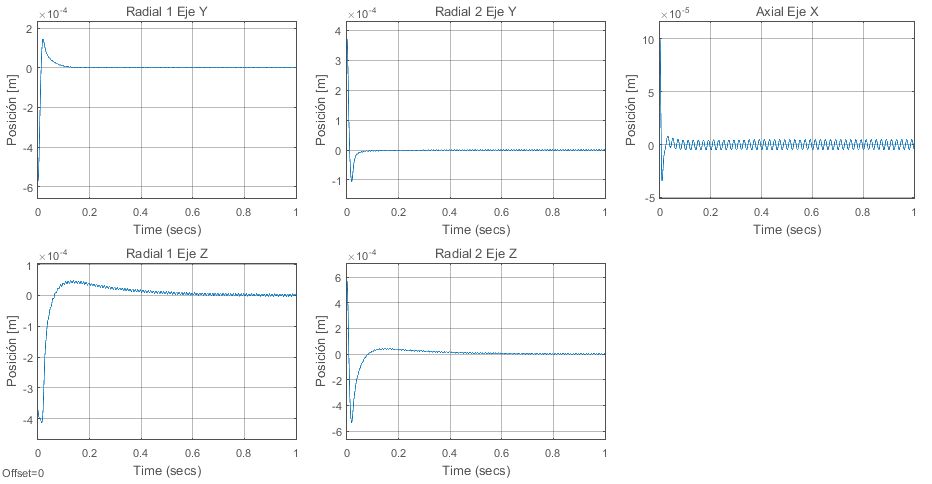
\includegraphics[width=\textwidth]{images/Capitulo_4_resultados_simulacion/simu_mcce_respuesta_carga_combinada}
\caption{Simulaci�n con carga combinada.}
\label{fig:Simulacion_carga_combinada}
\end{center}
\end{figure}

Se simulan el control calendarizado discreto integral y observador calendarizado discreto 

la simulacion empieza con condiciones iniciales de ...

se aplica una carga compuesta de ...

a diferencia de las simulaciones pasadas se retroalimenta la se�al de control del MCCE con la magnitud de la componente de fuerza en el eje $Z$  

se simulan dos situaciones : la uno es con el MCCE activado y la otra con el MCCE desactivado 

en cuanto a la salida del sistema (posici�n del eje) el resultado de la simulacion activada es el de la figura \ref{fig:Simulacion_MCCE_activado}

\begin{figure}[H]
\begin{center}
\centering
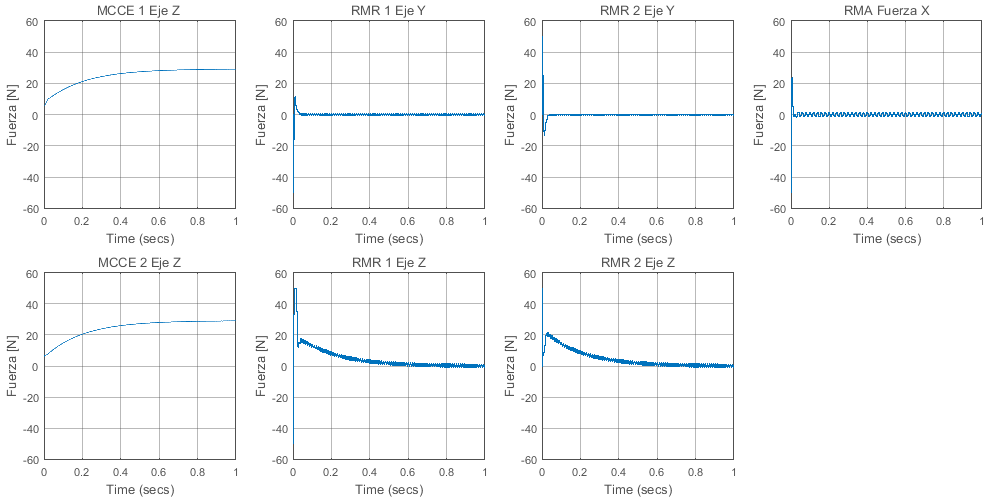
\includegraphics[width=\textwidth]{images/Capitulo_4_resultados_simulacion/simu_mcce_fuerzas_activo}
\caption{Simulaci�n con MCCE activado.}
\label{fig:Simulacion_MCCE_activado}
\end{center}
\end{figure}

con la simulacion desactivada el resultado en la salida del sistema es la figura \ref{fig:Simulacion_MCCE_desactivado}

\begin{figure}[H]
\begin{center}
\centering
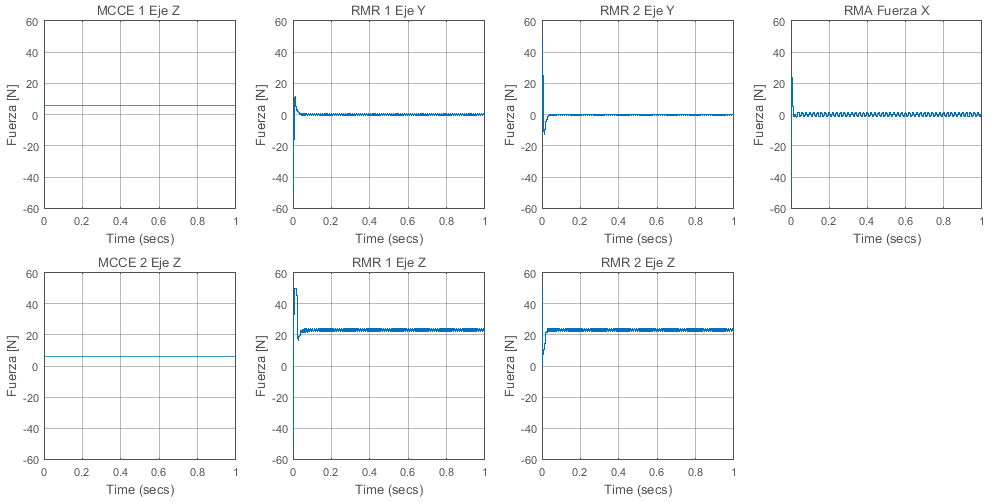
\includegraphics[width=\textwidth]{images/Capitulo_4_resultados_simulacion/simu_mcce_fuerzas_desactivado}
\caption{Simulaci�n con MCCE desactivado.}
\label{fig:Simulacion_MCCE_desactivado}
\end{center}
\end{figure}

se puede apreciar que activar el lazo de control de MCCE no compromete la estabilidad del sistema 

podemos comparar las fuerzas aplicadas por cada rodamiento en la figura [...] 

\textbf{[figuras de fuerzas]}

aqui podemos ver que cuando el MCCE est� desactivado el $RMR_z$ mantiene una fuerza de (20 N) una vez el sistema se ha estabilizado, mientras que el MCCE mantiene la fuerza m�nima del im�n permanente de (6 N)

cuando podemos ver que cuando el MCCE est� activado el $RMR_z$ mantiene una fuerza de (0 N) una vez el sistema se ha estabilizado, mientras que el MCCE mantiene la fuerza m�nima del im�n permanente de (26 N)
